\documentclass[leqno,presentation]{beamer}
\DeclareGraphicsExtensions{.eps,.jpg,.png,.tif}
\usepackage{amssymb, amsmath, pdfpages, amsfonts, calc, times, type1cm, latexsym, xcolor, colortbl, hyperref, bookmark}
\usepackage{graphicx}
\usepackage{tabularx}
\usepackage{multirow}
\graphicspath{ {images/} }

\usepackage[latin1]{inputenc}
\usepackage[english]{babel}
\usetheme{Darmstadt}
\newcommand{\R}{\mathbb{R}}
\newcommand{\N}{\mathbb{N}}
\newcommand{\overbar}[1]{\mkern1.5mu\overline{\mkern-1.5mu#1\mkern-1.5mu}\mkern1.5mu}
\newcommand{\highlight}[1]{
  \addtolength{\fboxrule}{.2ex}
  \begin{block}{}
    \begin{quote}#1
    \end{quote}
  \end{block}
}
\title{Automata and Numeration Systems}
\author[names]{Eric Ma, Reed Oei, Steve O'Brien, Dagoberto Saenz, Mihika Poddar \\ Eion Blanchard and Alexi Block Gorman (Team Leaders) \\ Erik Donal Walsberg and Philipp Hieronymi (Faculty mentors)}

\institute{
  \\[-3ex]
  University of Illinois at Urbana-Champaign
  \\[2ex]
  \includegraphics[width = 0.3\textwidth]{UIUC_logo.png}
  \hspace{.30cm}
  
\includegraphics[width = 0.07\textwidth]{igl-logo-small.png}
  \\[3ex]
  Illinois Geometry Lab  \\  Midterm Presentation\\ March 13, 2019\\[2ex] }


\title{Automata and Numeration Systems}

\date{}

\begin{document}
% Title slide
\frame{\titlepage}

% Slide 2
\section{Numeration Systems}
\begin{frame}
  
  \frametitle{Numeration systems}
  
  \begin{itemize}
  \item Method of representing quantities
  \item Base ten:
  \end{itemize}
  
%   \vspace{}
  
  \center{$\overbar{\ldots \text{dcba}} = \textcolor{red}{1} \cdot \text{a } + \textcolor{red}{10} \cdot \text{b } + \textcolor{red}{100} \cdot \text{c } + \textcolor{red}{1000} \cdot \text{d } + \ldots$}
  
%   \vspace{}
  
  \begin{itemize}
  \item Fibonacci numeration system utilizes the Fibonacci sequence (1, 2, 3, 5, 8, 13, ...):
  \end{itemize}
  
%   \vspace{}
  
  \center{$\overbar{\ldots \text{dcba}} = \textcolor{red}{1} \cdot \text{a } + \textcolor{red}{2} \cdot \text{b } + \textcolor{red}{3} \cdot \text{c } + \textcolor{red}{5} \cdot \text{d } + \ldots$}
  
  
\end{frame}


% Slide 3
\begin{frame}
  
  \frametitle{$\sqrt{2}$-Ostrowski numeration system}
  
  \begin{itemize}
  \item {The $\sqrt{2}$-Ostrowski numeration system utilizes the continued fraction expansion of $\sqrt{2}-1$}
  \item {Each place in the numeration system is defined recursively as:}
  \end{itemize}
  \center{$q_{\text{ -1}} = 0, q_{\text{ 0}} = 1, q_{\text{ k + 1}} = 2q_{\text{ k}} + q_{\text{ k - 1}}$}
  
  
  \begin{itemize}
  \item We get $q_{\text{ 0}} = 1, q_{\text{ 1}} = 2, q_{\text{ 2}} = 5, q_{\text{ 3}} = 12, \ldots$
  \item E.g. $21 = \textcolor{red}{12} \cdot 1 + \textcolor{red}{5} \cdot 1 + \textcolor{red}{2} \cdot 2 + \textcolor{red}{1} \cdot 0 = (1120)_{\sqrt{2}}$
  \end{itemize}
  
\end{frame}

\section{Automata}
% Slide 4
\begin{frame}
  \frametitle{Automata}
  \begin{itemize}
  \item {A finite state automaton is a machine that either accepts or rejects an input. It can be represented as a collection of states and transitions.}
  \end{itemize}
%   \vspace{}
  \center{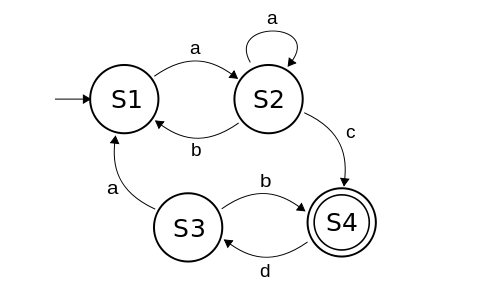
\includegraphics[width=.65\textwidth]{images/Automata.png}}
%   \vpsace{}
\end{frame}

% Slide 5
\begin{frame}
  \frametitle{Evaluating an automata example}
  \begin{tabular}{cl}
    \begin{tabular}{c}
      \parbox{0.5\linewidth}{
          Acceptable input \begin{itemize}
          \item $30 = 1 + 29$
          \item $30_{10} = {10001}_{\sqrt{2}}$
          \item lsd: $1,0,0,0,1$
          \end{itemize}
          %vspace{}
          Rejected input \begin{itemize}
          \item $30 = 1 + 5 + 2 \times 12$
          \item $30_{10} = {2101}_{\sqrt{2}}$
          \item lsd: $1,0,1,2$
          \end{itemize}
        }
    \end{tabular}
    & \begin{tabular}{l}
        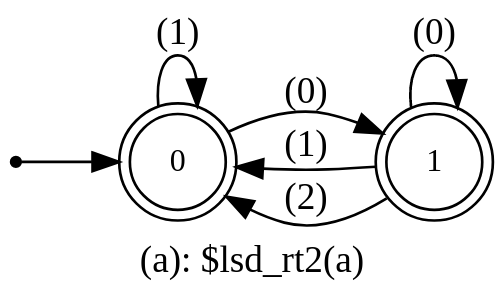
\includegraphics[width=.45\textwidth]{images/lsd_rt2.png}
      \end{tabular}
  \end{tabular}
\end{frame}

\section{Sturmian Words}
% Slide 6
% \begin{frame}
%   \frametitle{Walnut}
%   Walnut is a software package that allows us to decide certain combinatorial properties of some special words or predicates. It supports a lot of algebraic and logical operators and it can generate an automaton for the given predicates in any numeration system we define.
% \end{frame}

% % Slide 7
% \begin{frame}
%   \frametitle{Example of automata generated by Walnut}
%     \begin{tabular}{cl}
    
%     \begin{tabular}{c}
    
%       \parbox{0.5\linewidth}{
%         \texttt{eval add\_one "b=a+1"}\\
        
%         This evaluates to an automaton with 2 inputs labeled a and b. The automaton reads a and b from the least significant digit in binary numeration system and accepts only if $\text{b} = \text{a} + 1$.
%         }
%     \end{tabular}
%     & \begin{tabular}{l}
%          \includegraphics[width=.45\textwidth]{g.JPG}
%       \end{tabular}
%   \end{tabular}
% \end{frame}

% % Slide 8
% \begin{frame}
%   \frametitle{Defining numeration systems}
%   To define a numeration system using Walnut we need three automata:
%   \begin{itemize}
%   \item {verification}
%   \item {addition}
%   \item {comparison (automatically generated)}
%   \end{itemize}
%   %vspace{}
%   \begin{columns}
%       \begin{column}{0.25\textwidth}
%             \includegraphics[height=.4\textheight]{Capture.JPG}\\
%             \centerline{\hspace{1.7cm}$\text{Verify}_{fib}$}
%     \end{column}
%     \begin{column}{0.4\textwidth}
%         \includegraphics[height=.4\textheight]{image1.JPG}\\
%         \centerline{\hspace{1.7cm}$\text{Addition}_{fib}$}
%     \end{column}
%   \end{columns}
% \end{frame}

\begin{frame}
    \frametitle{Sturmian Words}
    
    \begin{itemize}
        \item Imagine hitting a billiard ball at some angle $\theta$
        \item When the ball crosses a vertical line, write a 0; for horizontal lines, write a 1
        \item Each $\theta$ defines a \textit{characteristic Sturmian word}
        \item $C_\phi = 0100101001\ldots$
    \end{itemize}
    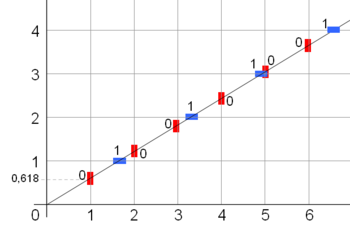
\includegraphics[height=0.5\textheight]{images/Fibonacci_word_cutting_sequence.png}
\end{frame}

\begin{frame}
    \frametitle{Generating Sturmian Words}
    \begin{itemize}
        \item To calculate $C_{\sqrt{2}}[N]$:
            \begin{itemize}
                \item Write $N$ in Ostrowski-$\sqrt{2}$
                \item Count the number trailing of $0$s, $\#_0(N)$
                \item $C_{\sqrt{2}}[N] = \#_0(N) \mod{2}$
            \end{itemize}
    
        \item $2 = 10_{\sqrt{2}} \mapsto 1$
        \item $102 = 110011_{\sqrt{2}} \mapsto 0$
    \end{itemize}
    
    \begin{figure}
        \centering
        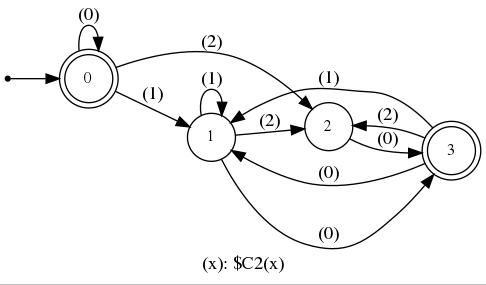
\includegraphics[height=0.5\textheight]{images/c2.jpg}
        \caption{An automaton that outputs $C_{\sqrt{2}}$}
        \label{fig:c2}
    \end{figure}
\end{frame}

\section{Progress}
% Slide 9
% \begin{frame}
%   \frametitle{What we have done}
%   \begin{itemize}
%   \item {Created addition automaton in $\sqrt{2}$ Ostrowski numeration system}
%   \item {We needed three individual automata to achieve this}
%   \item {After some struggle, we wrote a program to produce the automata (first automaton contains a total of 11,644 states)}
%   \end{itemize}
%   \begin{columns}
%     \begin{column}{0\textwidth}
%         \includegraphics[height=.4\textheight]{alg_1_1.JPG}
%     \end{column}
%     \begin{column}{0.1\textwidth}
%         \includegraphics[height =.4\textheight]{alg_1_2_1.JPG}
%     \end{column}
%   \end{columns}
% \end{frame}

% % Slide 10
% \begin{frame}
%   \frametitle{Automaton 1}
%   \includegraphics[width=\linewidth, height=.75\textheight]{testAlg1.JPG}
% \end{frame}

% Slide 11
\begin{frame}
  \frametitle{Programming the algorithms instead}
  \begin{itemize}
 \item{Walnut is an automated prover}
  \item {Walnut is able to effectively produce an automaton which only includes the necessary states and transitions}
  \item {By writing predicates into walnut, the program is able to produce an automaton}
  \end{itemize}
\end{frame}

\begin{frame}
  \frametitle{Programming the algorithms instead}
   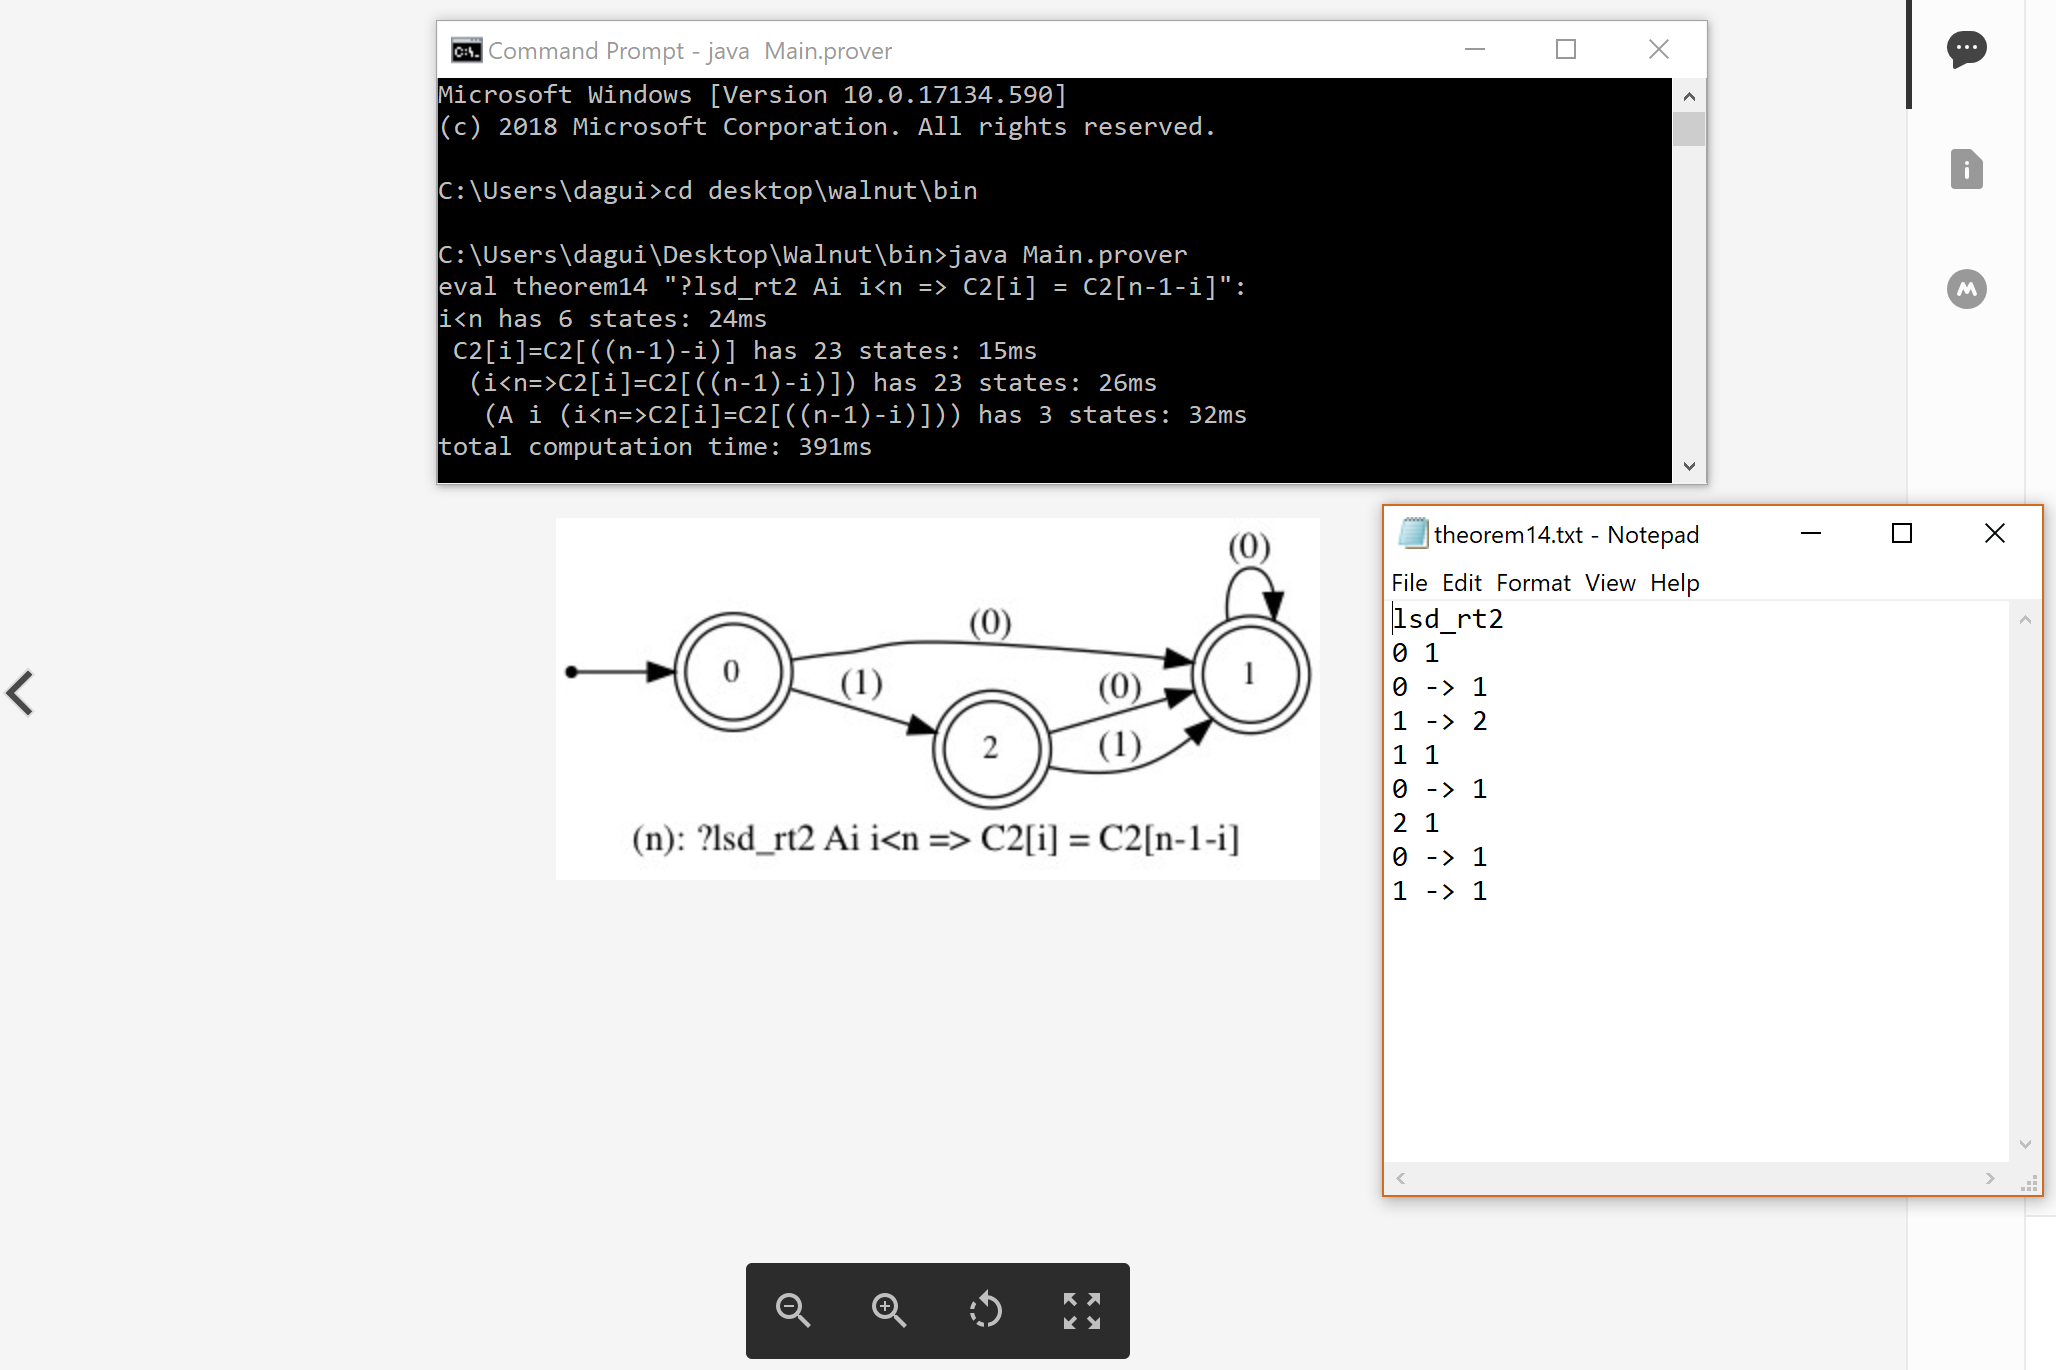
\includegraphics[width=\linewidth]{Walnut.png}
\end{frame}

\begin{frame}
  \frametitle{Example Theorems}
  Let $C_{\sqrt{2}}$ be the Sturmian word with slope $\sqrt{2}-1$.\\
  \vspace{1em}
%   \begin{table}[]
      \begin{tabularx}{\textwidth}{Xl}
      Theorem: $C_{\sqrt{2}}$ contains only anti-squares of order 1,2,3, and 4. \newline\texttt{\footnotesize?msd\_rt2 Ei Ak k<n => (C2[i+k] != C2[i+k+n])} & \raisebox{-0.9\height}{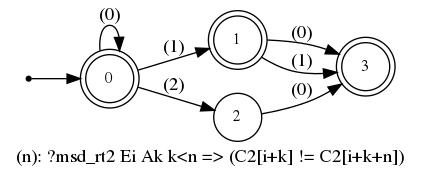
\includegraphics[width=0.5\linewidth]{theorem11.jpg}}  \\
      \hline
          \vspace{0em}Theorem: $C_{\sqrt{2}}$ contains no fifth power. \newline\texttt{\footnotesize?msd\_rt2 ((n> 0) \& (Ei At (t < 4 * n => C2[i+t] = C2[i+n+t])))}& \raisebox{-1.5\height}{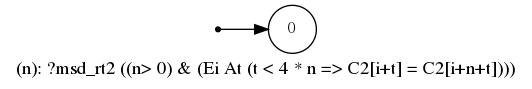
\includegraphics[width=0.5\linewidth]{theorem5_1.jpg}}
      \end{tabularx}
%   \end{table}
%   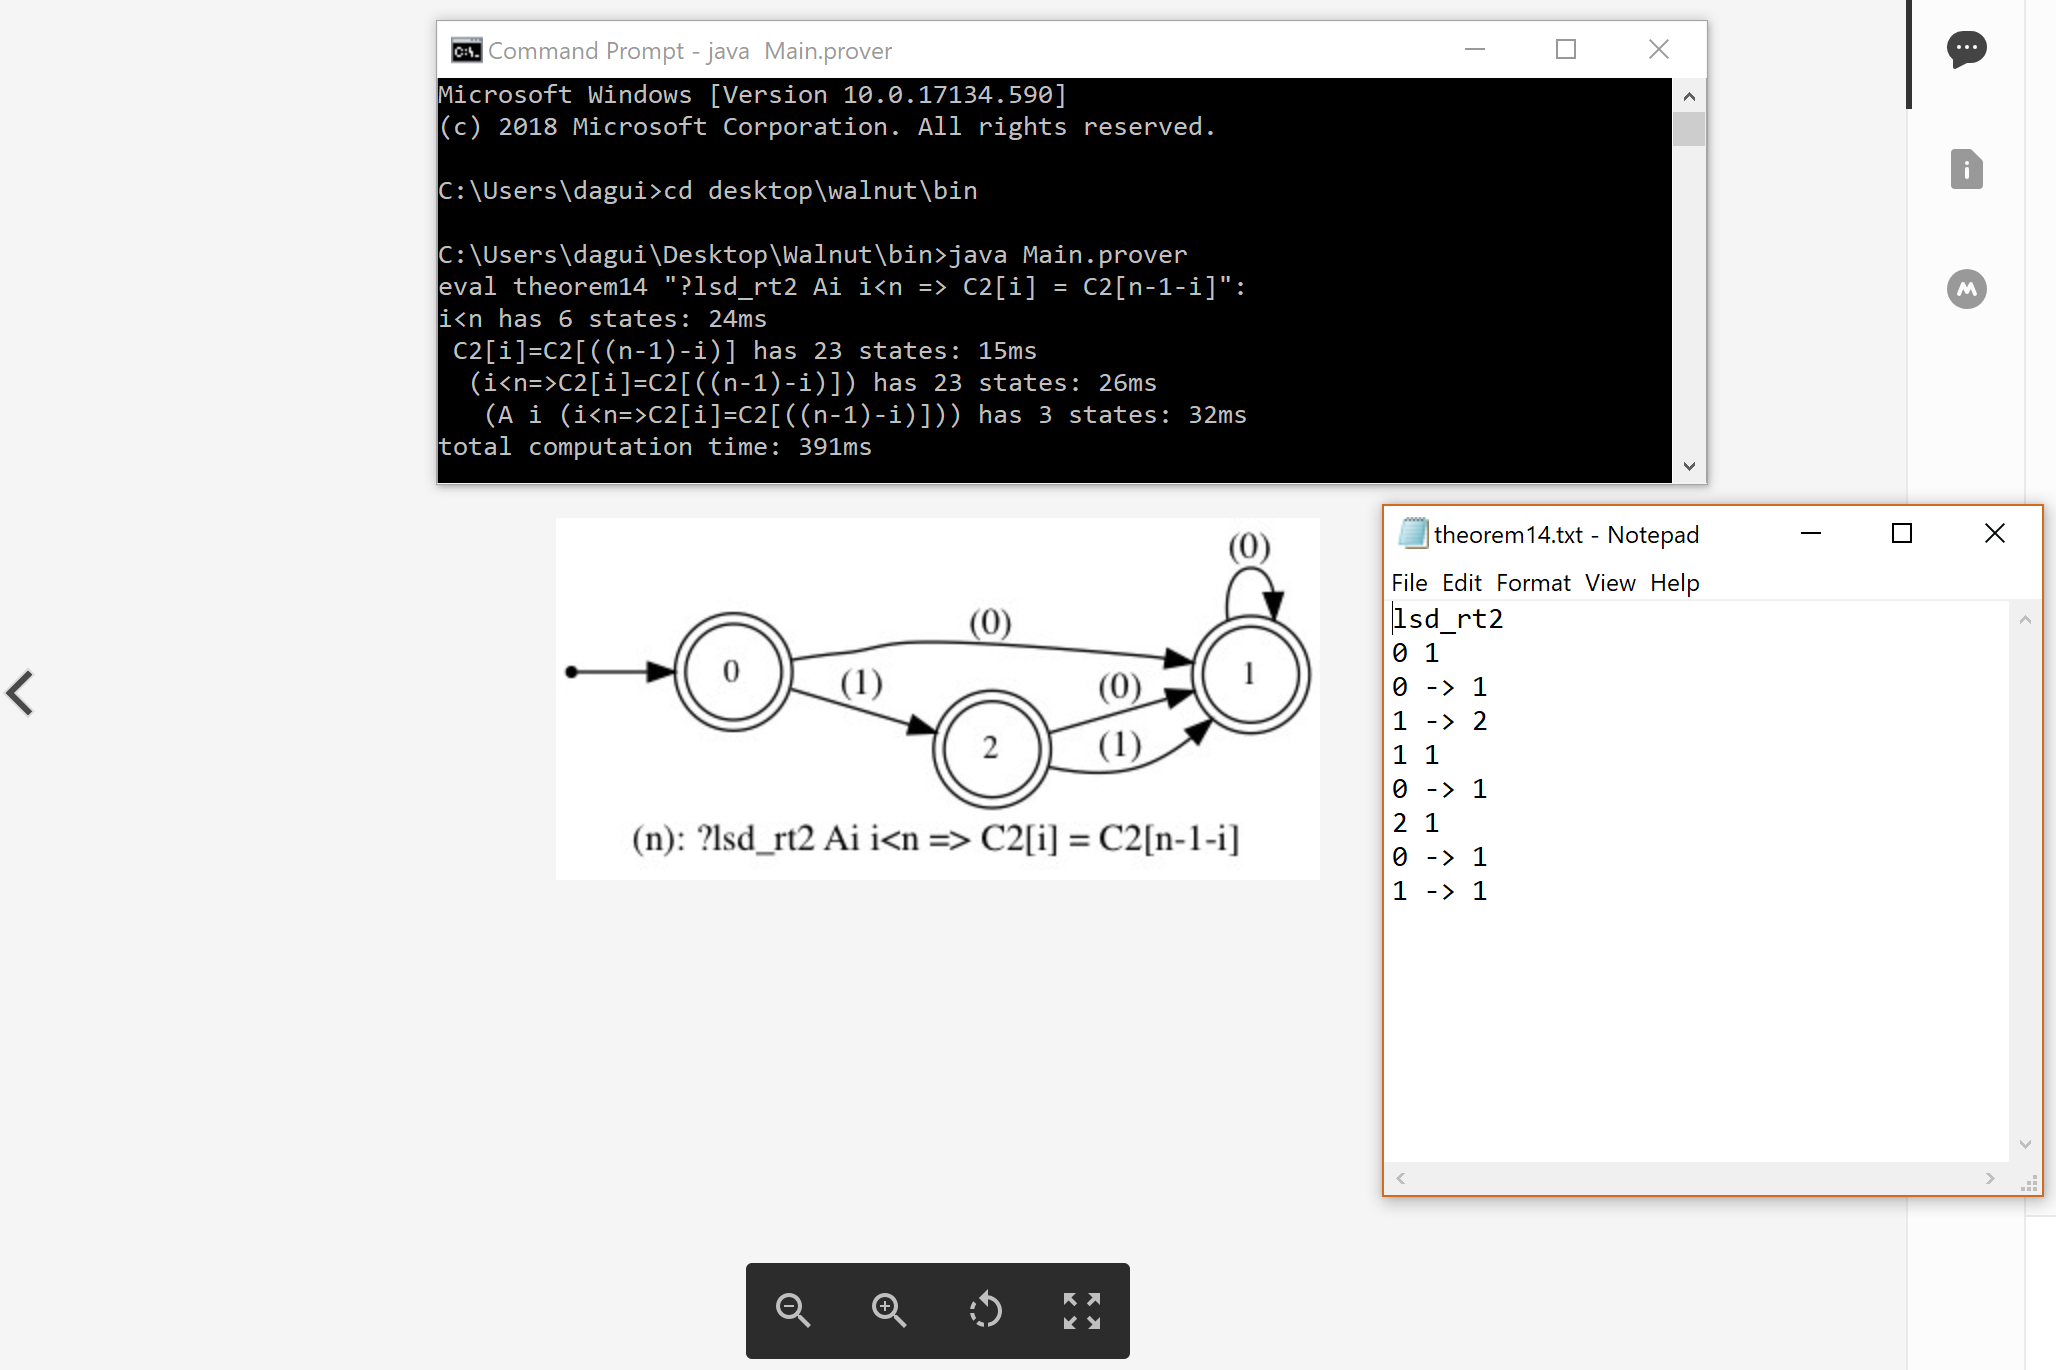
\includegraphics[width=\linewidth]{Walnut.png}
\end{frame}

% Slide 12
% \begin{frame}
%   \frametitle{Final automaton for addition in $\sqrt{2}$ Ostrowski}
%   \includegraphics[width=\linewidth, height=.75\textheight]{lsd_rt2_addition.JPG}
% \end{frame}

\section{Future Work}
% Slide 13
\begin{frame}
  \frametitle{Future work}
  \begin{enumerate}
  \item Generate characteristic Sturmian words with slope other than $\sqrt{2}-1$ (e.g. $\sqrt{3}-1 = [\overline{1,2}]$), and give Walnut theorems about the words to evaluate, and potentially write a paper for it.
  
  \item We already have a program to generate addition and recognition automata given any quadratic irrational number. We want to modify our program so that it can produce addition automata that takes the quadratic irrational number as an input.

  \end{enumerate}
  
\end{frame}
\begin{frame} %%%%%%%%% Make it Larger/typeset it %%%%%%%%%%
  \frametitle{Future work}
  

    
    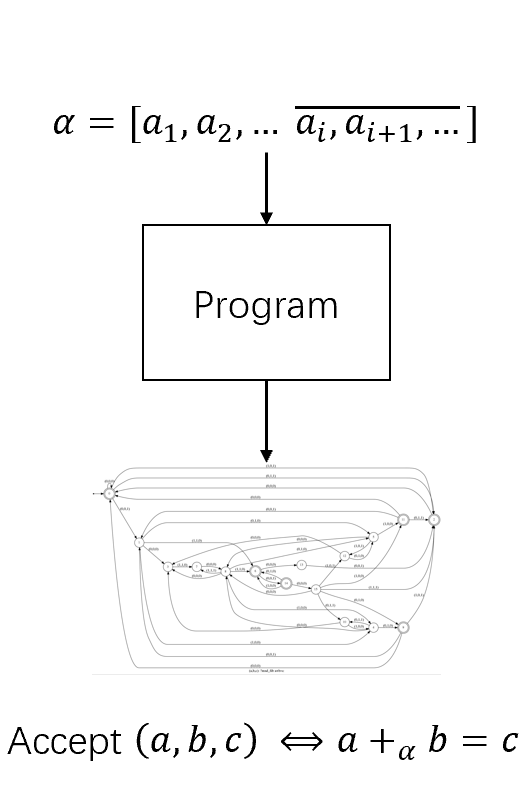
\includegraphics[width=0.31\linewidth]{future10.png}
    \hspace{5pt}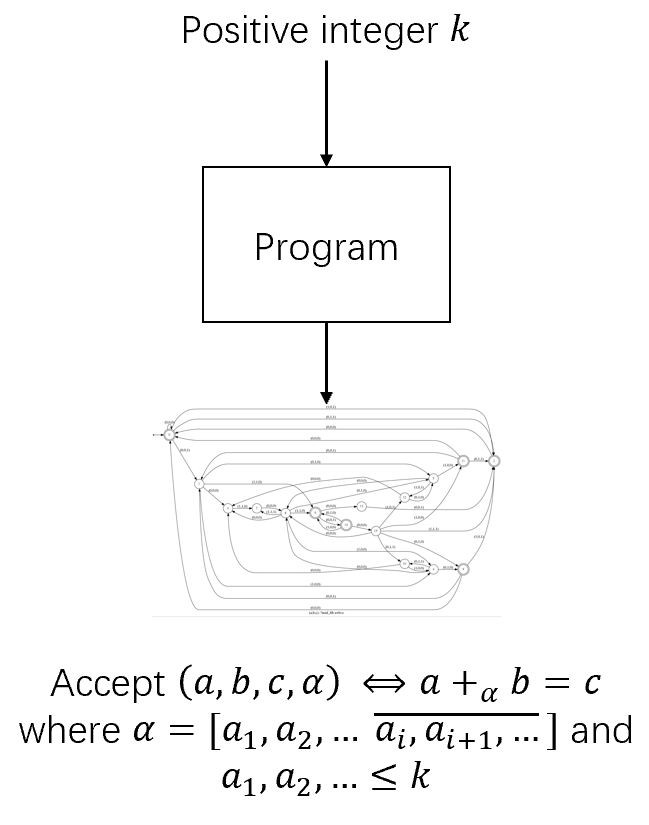
\includegraphics[width=0.32\linewidth]{future11.png}
    % 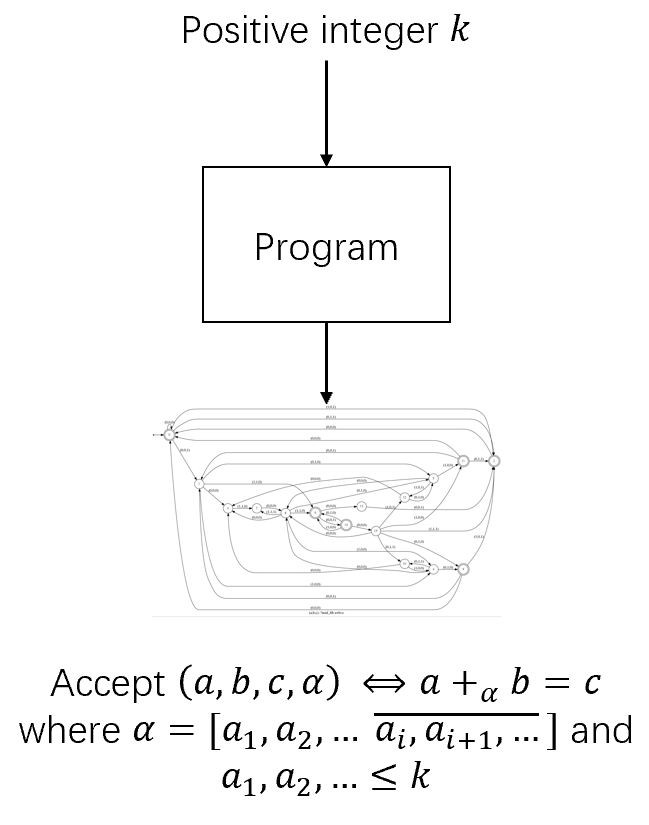
\includegraphics[width=0.33\linewidth]{future11.png}
   \hspace{5pt} 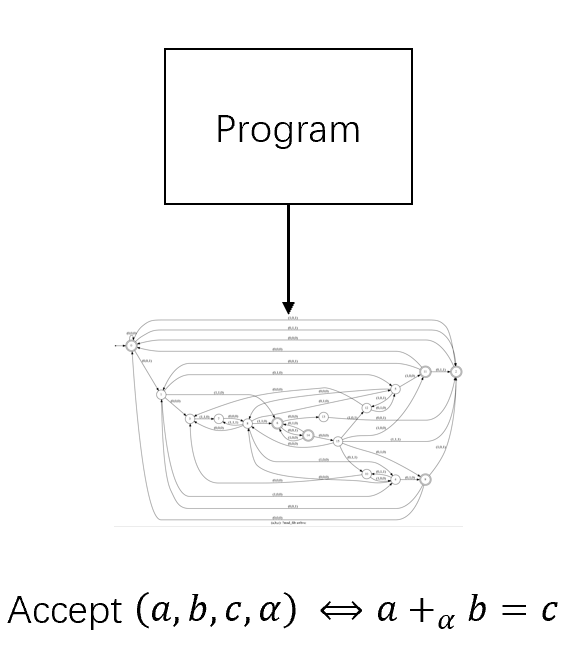
\includegraphics[width=0.31\linewidth]{future12.png}

    
\end{frame}

\end{document}